% -*- TeX-master: "../fat_manual.tex" -*-

\section{RHUL VNA Rohde and Schwartz}
An  important parameter  is  \textbf{IF Bandwidth  (Resolution Bandwidth,  RBA)}
which measures what frequency range to capture around every point measured:

\begin{figure}[h]
  \centering \includegraphics[height=8cm]{vna/vna_if_bandwidth}
  \caption{\small If we take  a 4 GHz span starting at 8 GHz  and stopping at 12
    GHz with \textbf{801} measurements points, the resulting frequency step size
    is \textbf{5  MHz}.  If then  a measurement bandwidth  of 10 kHz  is chosen,
    there is a clear  gap where we have no coverage  of the measurement receiver
    and signals can be missed.\label{fig:vna/vna_if_bandwidth}}
\end{figure}

\begin{framed}\noindent
  \textbf{Make the step smaller than the bandwidth in order to get good overlap}

  For  finer measurement,  it  makes sense  to  use a  finer  bandwidth. If  the
  bandwidth is too small however.  1Hz - 1second per point. 100Hz - 0.01 seconds
  per point.
\end{framed}


\begin{itemize}
\item \quote{Sweep} \ira \quote{sweepTIme}: continuous = sweep, CW = single freq
  (when we kno
\item \texttt{Scale} \ira autoscale
\item \texttt{Span} \ira Center 10GHz, span 16 GHz;
\item \quote{Power BW AVG} to set power, bandwidth;
\item RF ON.
\item \red{When first connected via ethernet, run the \quote{rsvna-lv\_2\_42\_0}
    installer and run the \quote{Set OPC timeout.vi} with 300000ms = 300 seconds
    or larger  in the  program, so  that the  wait time  from the  VNA to  PC is
    increased.}
\end{itemize}

\paragraph{VNA}  compares  the  \textbf{phase}   and  \textbf{amplitude}  of  an
outgoing signal to the one fed into the system.

 \begin{figure}[h]
   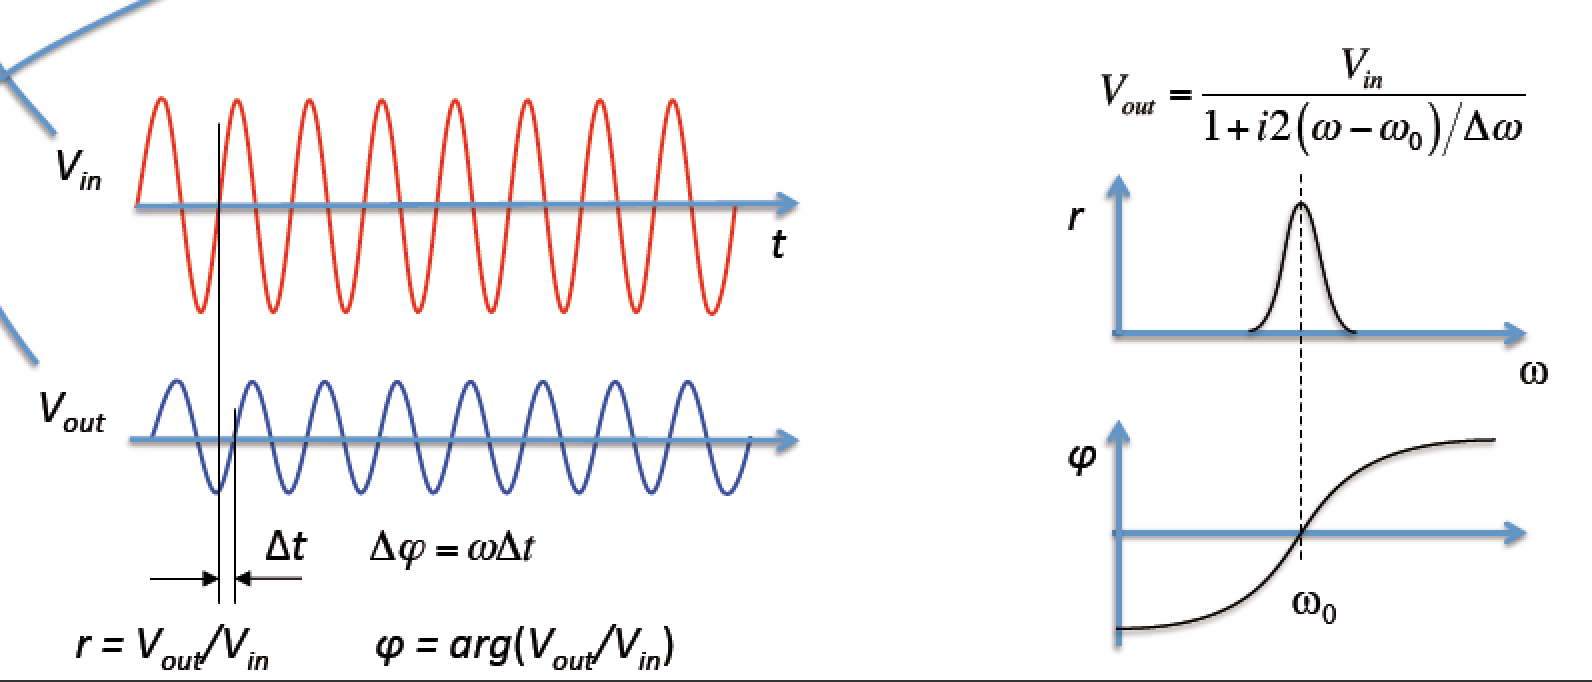
\includegraphics[height=4cm]{vna}
 \end{figure}

 \section{Trigger}
 \label{sec:trigger}

 For two tone measurement set \red{Trigger from sync}

 For Rabi set \red{Free run}

 \subsection{Correct phase}
 \label{sec:correct-phase}

 If  the  phase   is  choppy,  then  do   \cmd{click  \quote{Offset-embed}  \ira
   \quote{Auto-length}}.

 \begin{framed}\noindent
   There is also a program \textbf{Trigger-switch.vi} that can do it.
 \end{framed}

 \subsection{Measure Q factor}
 \label{sec:measure-q-factor}

 To measure q factor of resonator:
 \begin{enumerate}
 \item \cmd{Click \quote{Marker} and select 4 markers};
 \item \cmd{Click  \quote{Band filter} \ira \quote{Bandpass  reference to max}.}
   \red{make sure it's set to 3dB};
 \item  Markers will  be moved  to positions  where the  peak falls  off by  3dB
   (equivalent to halving) to work our the Q factor
 \end{enumerate}

 \subsection{Chopper}
 \label{sec:chopper}

 The chopper must be connected in the following configuration.

\begin{figure}[h]
  \centering \inkfig{8cm}{chopper_setup}
  \caption{\small Chooper  setup - otherwise there  will be bumps in  the signal
    pulses!\label{fig:chopper_setup}}
\end{figure}


\newpage
